\documentclass{beamer}
\usetheme{default}

\author{Michael Walker}
\title{A verified memory-management system for dynamic languages}
\institute{Department of Computer Science\\
  University of York\\
  \texttt{msw504@york.ac.uk}
}

\begin{document}

\begin{frame}[plain]
  \only<1>{\titlepage}
  % Hello, I'm Michael Walker, and my project was originally entitled
  % "A verified memory-management system for dynamic languages", but
  % it actually ended up just being about
  \only<2>{\centering \huge Verified Garbage Collection}
  % verified garbage collection in general.
\end{frame}

\begin{frame}{Overview}
  \tableofcontents
  % So I'll start by giving the motivation, and quickly introducing
  % the topics of garbage collection and software verification; and
  % then I'll go through what I did in this project: specifically,
  % determining what it means for various types of garbage collector
  % to be correct, looking at existing collectors as case studies, and
  % then generalising to produce a more widely-applicable definition
  % of correctness; and I'll conclude by evaluating the work, and just
  % briefly summarising the contributions again.
\end{frame}

%% Introduction

\section{Introduction}
\subsection{Motivation}

\begin{frame}{Motivation}
  \begin{itemize}
  \item Memory bugs can produce incorrect program results.
    \begin{itemize}
    \item The recent Heartbleed exploit in OpenSSL is a good (or bad)
      example of this.
    \end{itemize}

% Memory is hard to get right, and getting it wrong can have dire
% consequences. The recent Heartbleed exploit in OpenSSL is a good
% example of this: where a malicious user could request large amounts
% of encrypted text and an affected server would just happily hand it
% over, regardless of whether it should do or not. This isn't a
% garbage collection problem, but it did arise from a hard-to-find bug
% in an unverified memory management system. Naturally, we don't like
% this sort of thing happening.

  \item Can be hard to track down by hand.
  \item \textit{``testing shows the presence, not the absence of
      bugs''}
  \item Typically no formal verification, only testing.

% In a garbage collected program, the sorts of errors that could arise
% include freeing some memory whilst it is still needed, which could
% in the best case result in a crash, and the worst case an incorrect
% computation. However, it's easier to trust a garbage collector than
% it is to handle all of your memory yourself, and so garbage
% collectors have become a staple feature of modern programming
% languages, freeing the programmer to worry about more high-level
% concerns.

% Because memory is hard to get right, memory managers, like garbage
% collectors, tend to be complex, and it's often difficult to be sure
% they're right. Because of this, testing is widely used, but this
% isn't enough to guarantee correctness. The only way to be sure that
% there are no bugs is to construct a proof that the collector does do
% what it is supposed to do.
  \end{itemize}
\end{frame}

\subsection{Garbage Collection}

\begin{frame}{Garbage Collection}
  \only<1>{
    \begin{figure}[h!]
      \centering
      \includegraphics{heap1}
      \label{fig:heap1}
      \caption{No garbage: $A$ and $B$ reachable from the roots}
    \end{figure}
  }

% Garbage collection is the process of automatically removing
% unreachable memory from the heap, decreasing the memory usage of a
% program. If we consider the heap to be a digraph of memory cells
% connected by pointers, then the roots of this structure are the
% variables which are currently in scope: the stack.

  \only<2>{
    \begin{figure}[h!]
      \centering
      \includegraphics{heap2}
      \label{fig:heap2}
      \caption{$A$ becomes garbage when one of the roots is changed to
        point at $B$.}
    \end{figure}
  }

% A cell might become garbage when roots change, or when another cell
% is mutated. If a cell is garbage, it's useless. We don't want it any
% more. We'd much rather reduce the heap to

  \only<3>{
    \begin{figure}[h!]
      \centering
      \includegraphics{heap3}
      \label{fig:heap3}
      \caption{Remove $A$, so the heap is now minimal.}
    \end{figure}
  }

% this, as it's smaller.
\end{frame}

\begin{frame}{Garbage Collection: Mark-Sweep and Copying}
  \begin{figure}[h]
    \centering
    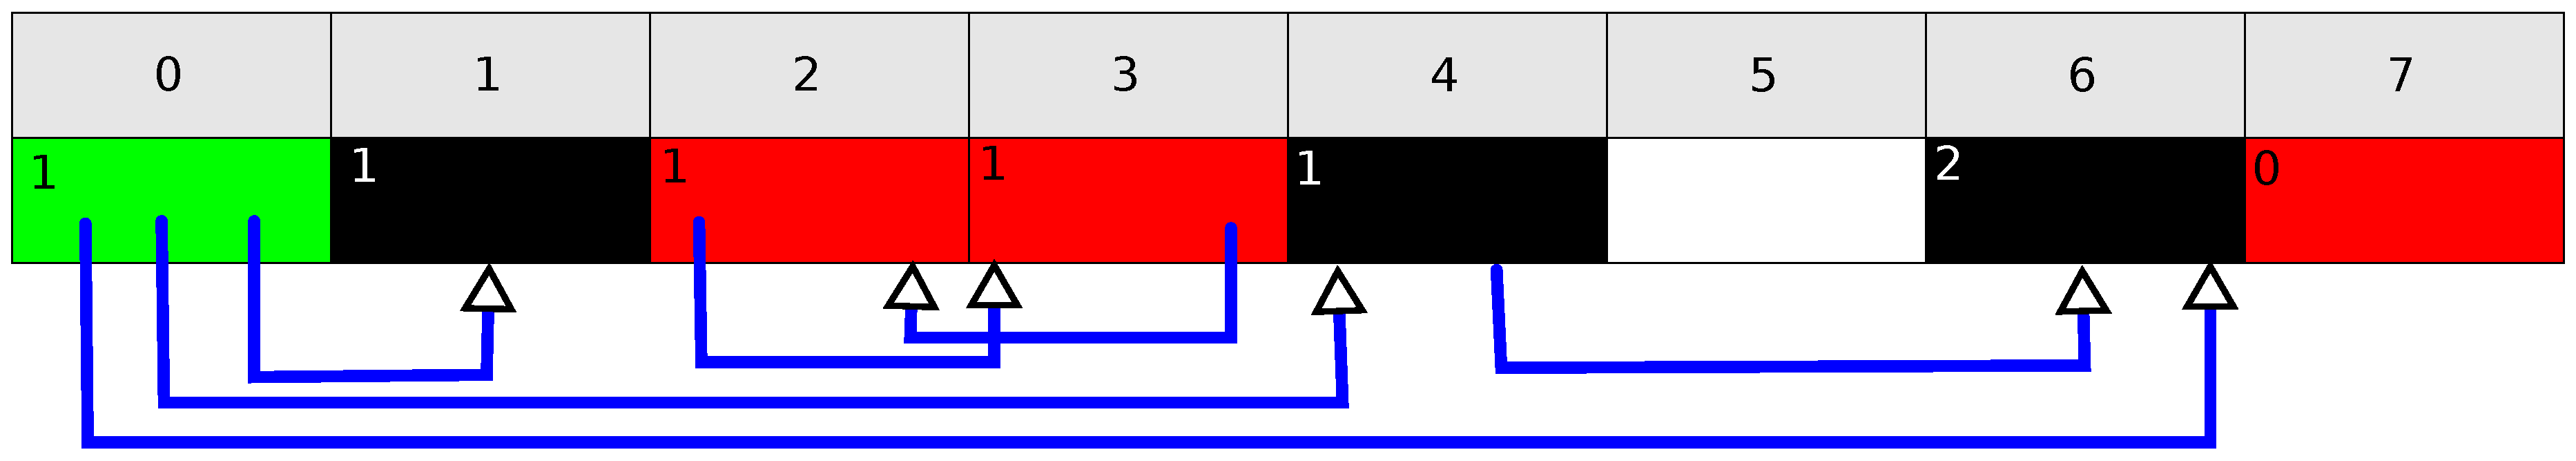
\includegraphics[width=\textwidth]{lit-gc-before}
    \caption{Heap before garbage collection}
    \label{fig:lit-gc-before}
  \end{figure}

% I'll be using a little example to explain the two types of garbage
% collector I considered: green cells are live, red are garbage, and
% white are free.

  \only<1>{
    \begin{figure}[h]
      \centering
      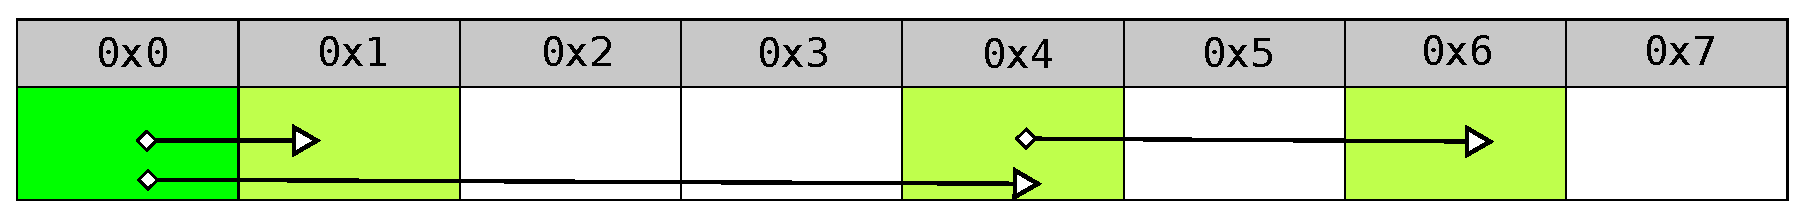
\includegraphics[width=\textwidth]{lit-gc-marksweep}
      \caption{Heap after mark-sweep collection}
      \label{fig:lit-gc-marksweep}
    \end{figure}

    \begin{itemize}
    \item Cells have a ``mark bit'', initially unset
    \item Heap is traversed from roots, setting mark bits (marking)
    \item Heap is traversed totally, freeing unmarked cells (sweeping)
    \item Removes all garbage
    \item Takes time proportional to the size of the heap
    \end{itemize}

% Mark-sweep collectors date from the early days of Lisp, and work by
% assigning to every cell a mark bit, which is initially unset. Upon
% running out of memory, the heap is traversed from the roots, and
% every cell reached has the mark bit set. Then the heap is traversed
% again, but this time the entire heap is traversed, and all marked
% cells are unmarked, and all unmarked cells are freed. This gets rid
% of all garbage, it's nice and simple to implement, but takes time
% proportional to the size of the heap, regardless of how many cells
% actually survive.
  }

  \only<2>{
    \begin{figure}[h]
      \centering
      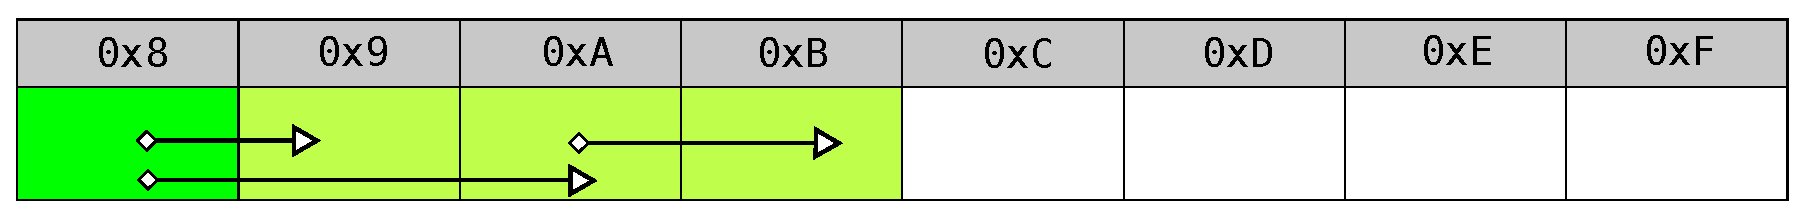
\includegraphics[width=\textwidth]{lit-gc-copying}
      \caption{Heap after copying collection}
      \label{fig:lit-gc-copying}
    \end{figure}

    \begin{itemize}
    \item Divides heap into two ``semispaces''
    \item Allocation only happens in one at a time
    \item At GC, live cells are copied to the other space, and the
      roles swapped
    \item Takes time proportional to size of the live portion of the
      heap
    \item Has a space cost of half the heap
    \item Potentially reduces cache misses and page faults.
    \end{itemize}

% Copying collectors are pretty different, they work by dividing the
% heap into two equal-sized pieces, in only one of which allocation
% happens. Upon running out of memory the heap is traversed from the
% roots, and all cells reached are copied to the other space and
% pointers updated, then allocation switches to happening in that
% space. This only takes time proportional to the size of the live
% portion of the heap, but it has a large space cost. However, by
% compacting the heap it improves locality of reference, and so can
% potentially have a side effect of reducing cache misses and page
% faults.
  }
\end{frame}

\subsection{Software Verification}

\begin{frame}{Software Verification}
  \begin{itemize}
  \item Produce a formal model from some code.
  \item Produce a formal model from a specification.
  \item Reason about the relation between the two.
  \end{itemize}

% Briefly, the idea behind software verification is that when you
% write some software, or at least the sort of software which you
% might want to verify, you don't just start going. You first produce
% a specification. Then, when you're done, you want to be sure that
% the code and the specification are actually talking about the same
% thing, but they're on totally different levels of abstraction, which
% complicates this. So what you do is you produce a formal model of
% how the code works, usually in terms of how it manipulates the
% program state, and a formal model of what the specification
% describes, and then use some logic to reason about the two.

% There's a slightly different way of approaching this, where you
% instead start from the formal specification, and keep producing
% slightly lower-level specifications until you get to code. If you
% have an unbroken chain of proofs, then by transitivity of
% refinement, you know that the top level specification and the code
% are equivalent, even if you haven't directly compared the two.

% Both approaches are good for different things.
\end{frame}

%% Contributions

\section{Contributions}
\subsection{Correctness of Garbage Collectors}

\begin{frame}{Correctness of Garbage Collectors}
\end{frame}

\subsubsection{Mark-Sweep}

\begin{frame}{Armstrong-Virding}
\end{frame}

\subsubsection{Copying}

\begin{frame}{Fenichel-Yochelson}
\end{frame}

\subsection{Generalising Correctness}

\begin{frame}{Generalising Correctness}
\end{frame}

%% Results

\section{Conclusions}
\subsection{Evaluation}

\begin{frame}{Evaluation}
\end{frame}

\subsection{Contributions}

\begin{frame}{Contributions}
\end{frame}

%% Presentation proper ends

\begin{frame}{Questions?}
  \centering \huge Questions?
\end{frame}

\end{document}